\documentclass[letterpaper,12pt]{article}
\usepackage[top=2cm, bottom=1.5cm, left=1cm, right=1cm]{geometry}
\usepackage{amsmath, amssymb, amsthm,graphicx}
\usepackage{fancyhdr}
\pagestyle{fancy}

\lhead{\today}
\chead{Logistic Growth}
\rhead{Justin Hood}

\newcommand{\Z}{\mathbb{Z}}
\newcommand{\Q}{\mathbb{Q}}
\newcommand{\R}{\mathbb{R}}
\newcommand{\C}{\mathbb{C}}
\newtheorem{lem}{Lemma}
\title{Logistic Growth}
\author{Justin Hood\\
MATH 710\\
Dr. Wojciechowski}

\begin{document}
\maketitle
\begin{abstract}
Logistic growth models have a wide variety of uses in the world of mathematical modeling and simulation. With applications ranging from ecology to machine learning, this seemingly simple differential equation form is capable of encoding an enormous amount of data within it. For this report, we will focus mainly on applications pertaining to population growth and control via a harvesting action. We will look at some numerical simulations of steady state solutions to the problem, as well as attempt to strip away some of the complexities of the differential equation to look at the mathematical underpinnings of how the different terms of the equation affect the overall solution.
\end{abstract}
\newpage
\section{Introduction}
We consider an equation describing Logarithmic Growth of a population with periodic harvesting from the population, based on the population size. Such an equation is,
\[\frac{dx}{dt}=s\bigg(1-\frac{x}{K}\bigg)x-hx\]
With $s$ being a ``rate constant", $K$ being the carrying capacity of the environment, and $h$ a unitless ``percentage" describing the harvesting from the population.
\subsection{Model Specifics}
For the purposes of this analysis, we consider a population of deer, with starting population $900,000$. The habitat that the deer live in has a capacity of $1,072,764$. A suitable reproductive rate constant for this population of deer is $.2311$. Thus, we may look at our specific differential equation,
\[\frac{dx}{dt}=.2311\bigg(1-\frac{x}{1072764}\bigg)x-hx\]
Our analysis for this model will pertain mainly to analyzing the different effects $h$ has on the population behavior.
\section{Harvesting's Effects}
Let us now consider the effects of different harvesting terms on the overall behavior of the population. Starting at $1\%$ and increasing incrementally to $5\%$, we see that the harvesting term acts to reduce the equilibrium population of the system. Consider below two examples with $h=.01$ on the left, and $h=.04$ on the right.\\
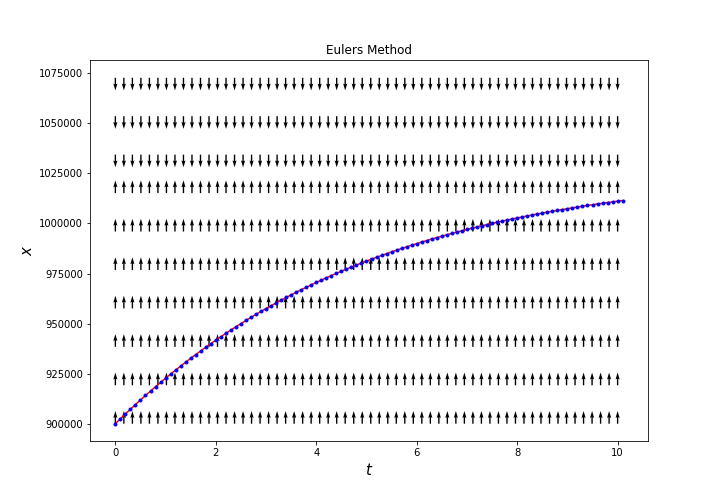
\includegraphics[scale=.4]{3a1.png}
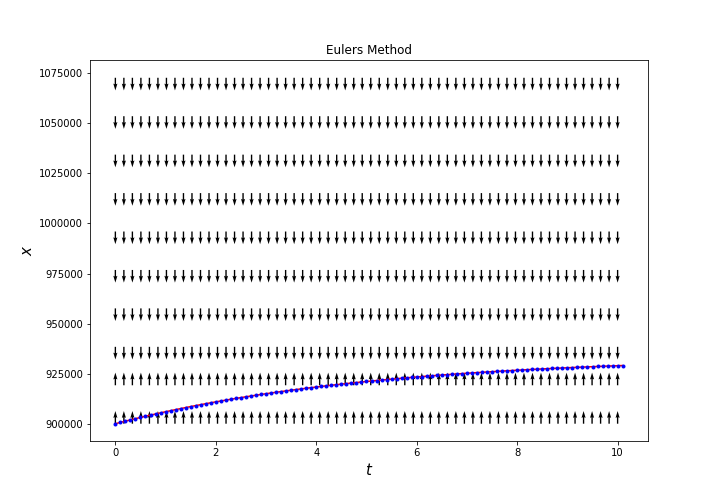
\includegraphics[scale=.4]{3a4.png}
We see that the solution curve with the higher harvesting rate has a lower long term population value. This leads to the obvious question, what are the equilibrium points of this model?
\section{Equilibria}
As we have in the past, we shall set the differential equation equal to zero, and solve for $x$ in order to obtain our steady state population values,
\begin{align*}
s(1-\frac{x}{K})x-hx &= 0\\
(s-h)x-\frac{s}{K}x^2 &= 0
\end{align*}
Substituting into the quadratic equation, we find the roots to be,
\[x=0,\ \frac{K(s-h)}{s}\]
So, the equilibrium points are zero, and a function of the different constants in our differential equation. 
\subsection{Point Behavior}
Considering the form of the non-zero equilibrium point, we note that as $h\to s$, the value of the equilibrium point will tend to zero. From this analysis, we may conclude that so long as $h<s$, the population will always tend towards a non-zero equilibrium point as defined by the root above. Should $h\geq s$, the population will decrease until it reaches extinction. To test this theory, we shall simulate the numeric solutions using the aforementioned constants $s$ and $K$, along with $h=\frac{s}{2},\text{and }h=s$. The plots follow.\\
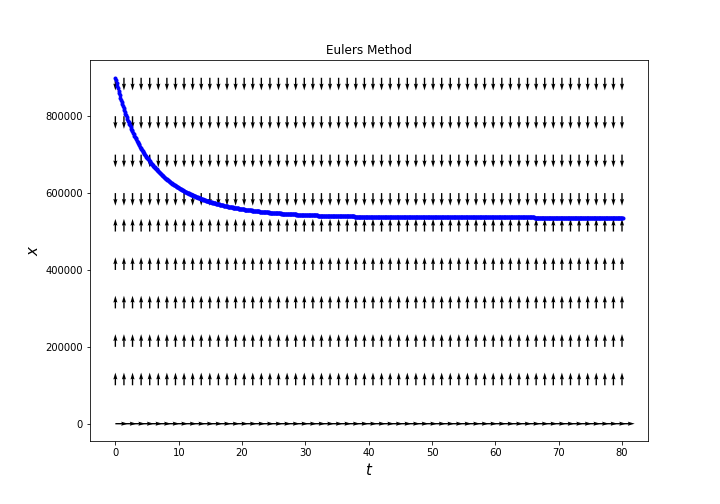
\includegraphics[scale=.4]{4b1.png}
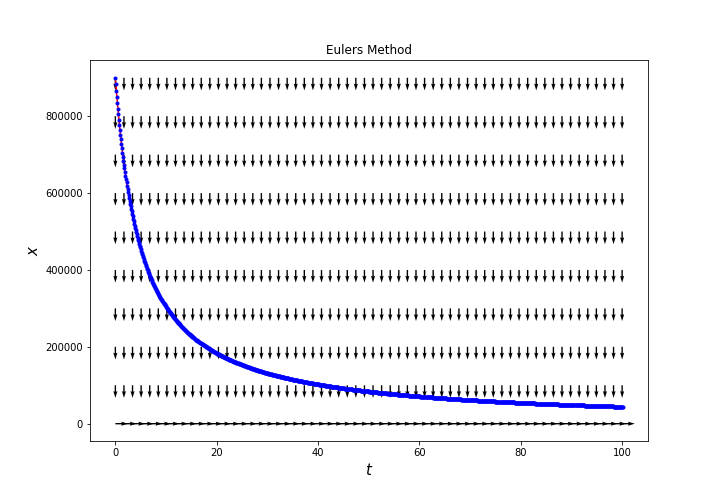
\includegraphics[scale=.4]{4b2.png}
On the left, we have $h=\frac{s}{2}$, and the right, $h=s$. As suggested by our analysis, the solution that tends to zero is the equation with $h=s$. It is perhaps worth noting as a point of curiosity that the solution with $h=\frac{s}{2}$ reaches a steady state at $\frac{K}{2}$.
\subsection{Changes in $s$}
From our above analysis, one could make the argument that $s$ is not a fixed value, as there are many random variables that come into play in computing it. As we change $s$, keeping $0\leq h<s$, we see the system exhibiting the same type of behavior as before, with only minor changes to concavity and slope for the solution curves.
\section{Population Control}
Using this newfound knowledge of the effect of $h$ on the equilibrium population value, we consider a situation wherein the population of deer needs to be controlled at a value lower than that of the carrying capacity of the environment itself. For instance, if the DNR wanted to maintain the deer population at $500,000$ in an effort to reduce disease spread and destruction of the habitat, they would need to hunt/harvest a certain amount of the deer each year. In order to compute this harvesting constant, we consider the following.\\\\
As previously described, we know that the ending equilibrium population is directly affected by $h$. As we have fixed both $s$ and $K$, we may solve the following relation to arrive at the critical $h$ value.
\begin{align*}
500000 &= \frac{K(s-h^*)}{s}\\
500000s &= Ks-Kh^*\\
Kh^* &= Ks-500000s\\
h^* &= \frac{Ks-500000s}{K}
\end{align*}
Substituting in the values of $s$ and $K$, we arrive at,
\[h^*=.123388\]
Thus, we see that the optimal harvesting rate is $\approx12.339\%$. So, the DNR would need to cull a little over $12\%$ of the deer population each year in order to keep the population on track to equilibrate at $500000$.
\section{Conclusion}
Overall, we have shown that each of the components of the differential equation that we have analyzed have an important role to play in determining the long term stable state behavior of the system. Whereas $K$ and $s$ have slightly more obvious definitions, meanings, and effects, we see that this harvesting term $h$ has the capability to send the population to extinction if allowed to grow unchecked. We have also seen how closely $h$ and $s$ are intertwined in terms of their creation and destruction of the population, due to the significance of their equality on the steady state solution to the system.
\newpage
Note: All associated python files are included, with appropriate commenting for further experimentation.
\end{document}
